\section{Appendix: The 14 composite spaces in $U$}
\label{chap:compositeCatalogue}

We here present the 14 spaces induced from g-blinks in $U$.
Their ``connected sum'' details: what prime spaces compose to
them are shown in Chapter~\ref{chap:census}. The elements of
this presentation are the same as the explained in
Appendix~\ref{chap:primeCatalogue}.

% \newcount\ii \newcount\jj   % declare integer variable
% \def\producePagesTwo#1#2{
% \ii=#1                      % initialize ii
% \jj=#2                      % initialize jj
% \advance\jj by 1            % increment jj
% \loop   % loop
%    \ifnum\ii<\jj
% {
%    %\vspace{-1cm}
%    %\thispagestyle{empty}
%    % \setlength{\hoffset}{0cm}
%    % \setlength{\textwidth}{\paperwidth-2cm}
%    \hspace{-1.8cm}
%    \enlargethispage{5cm}
%    {\centering
%    \includegraphics[height=23.5cm]{A.figs/compcatalog\ifnum\ii<100 0\fi\ifnum\ii<10 0\fi\number\ii.eps}
%    }
%    \newpage}
%       \advance\ii by 1
%    \repeat
% }

\newpage
\setlength{\topmargin}{-1.2cm}
%\setlength{\textwidth}{\paperwidth-2in}
%\setlength{\headheight}{1cm}
%\setlength{\headsep}{-3cm}
%\setlength{\footskip}{0.1cm}
%\setlength{\textheight}{\paperheight-\headheight-\headsep-\footskip-2in}
%\setlength{\oddsidemargin}{0mm}
%\setlength{\evensidemargin}{0mm}
%\setlength{\marginparwidth}{0mm}
%\setlength{\marginparsep}{0mm}
%\setlength{\textwidth}{\paperwidth-2in}

\begin{center}
 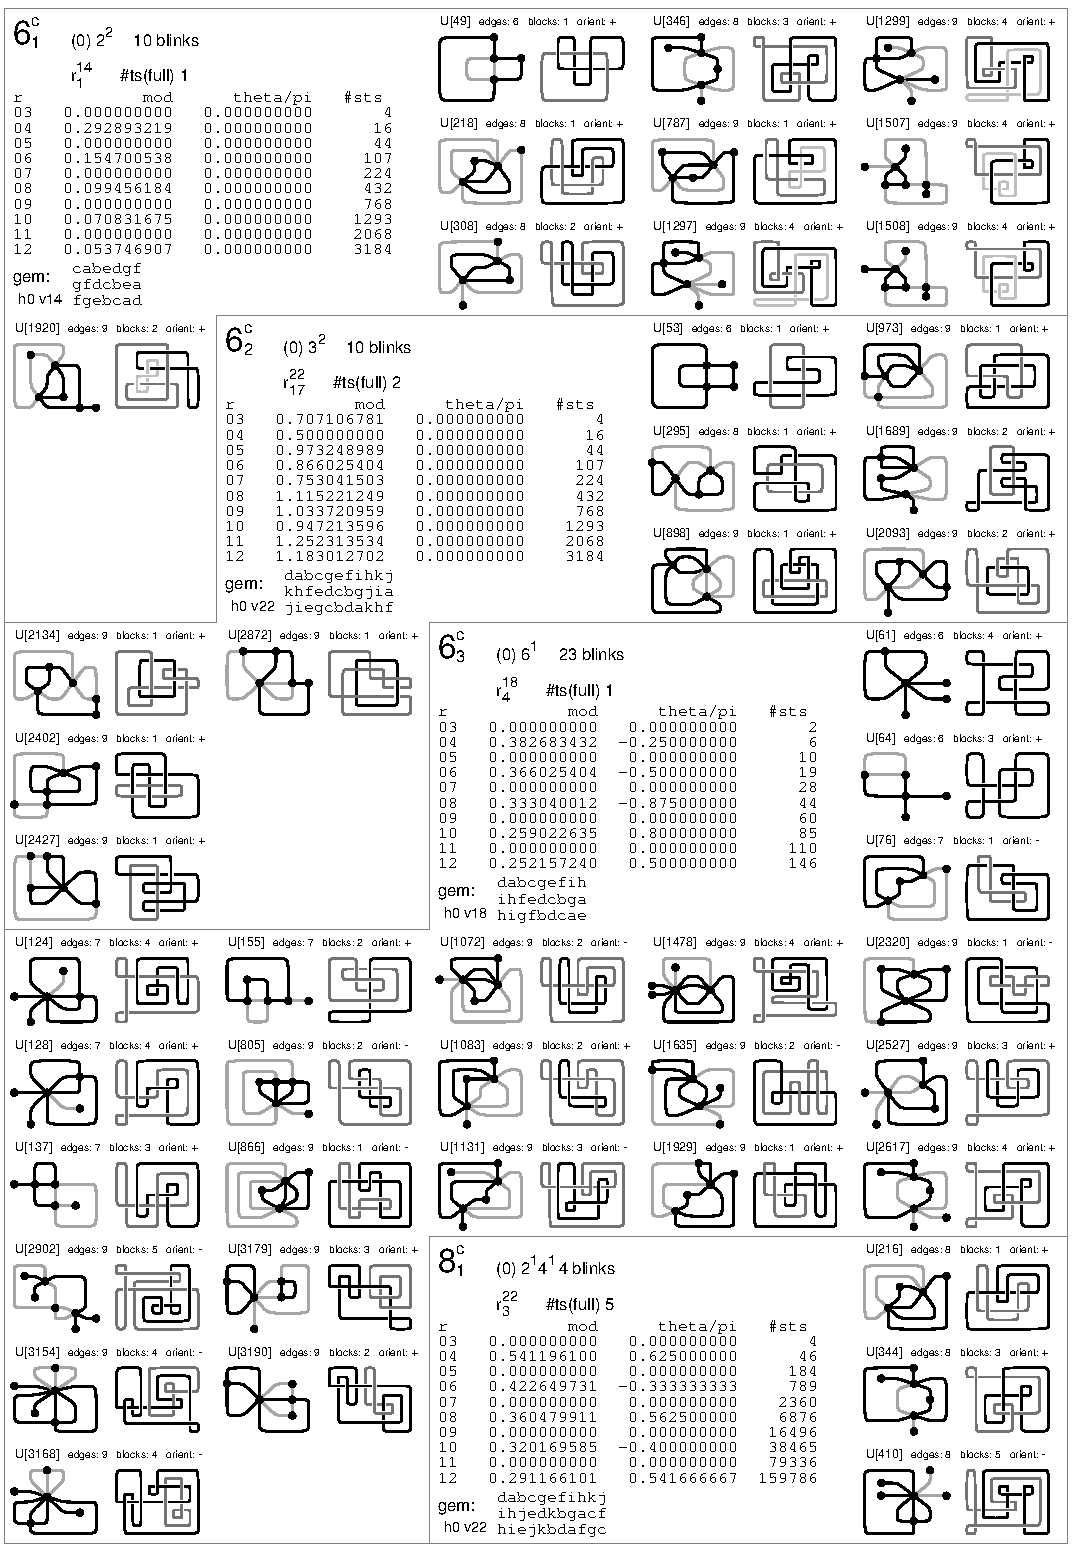
\includegraphics[height=23.5cm]{E.figsbw2/compcatalog001_bw.pdf} \eject
 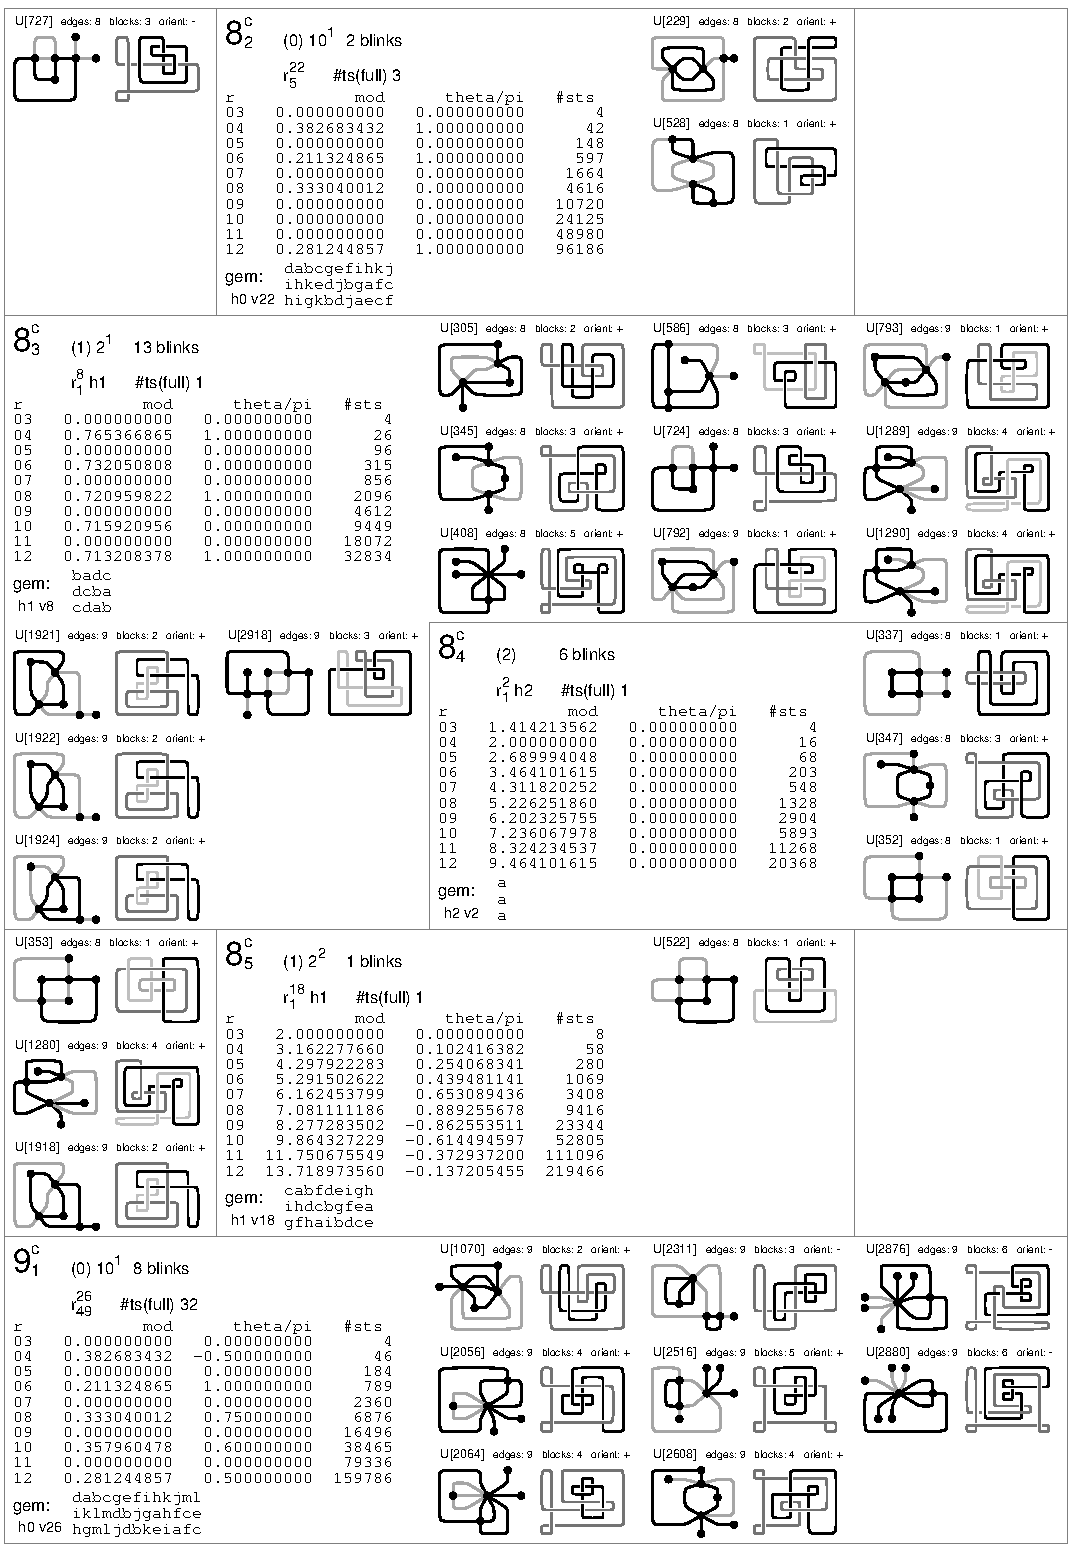
\includegraphics[height=23.5cm]{E.figsbw2/compcatalog002_bw.pdf} \eject 
 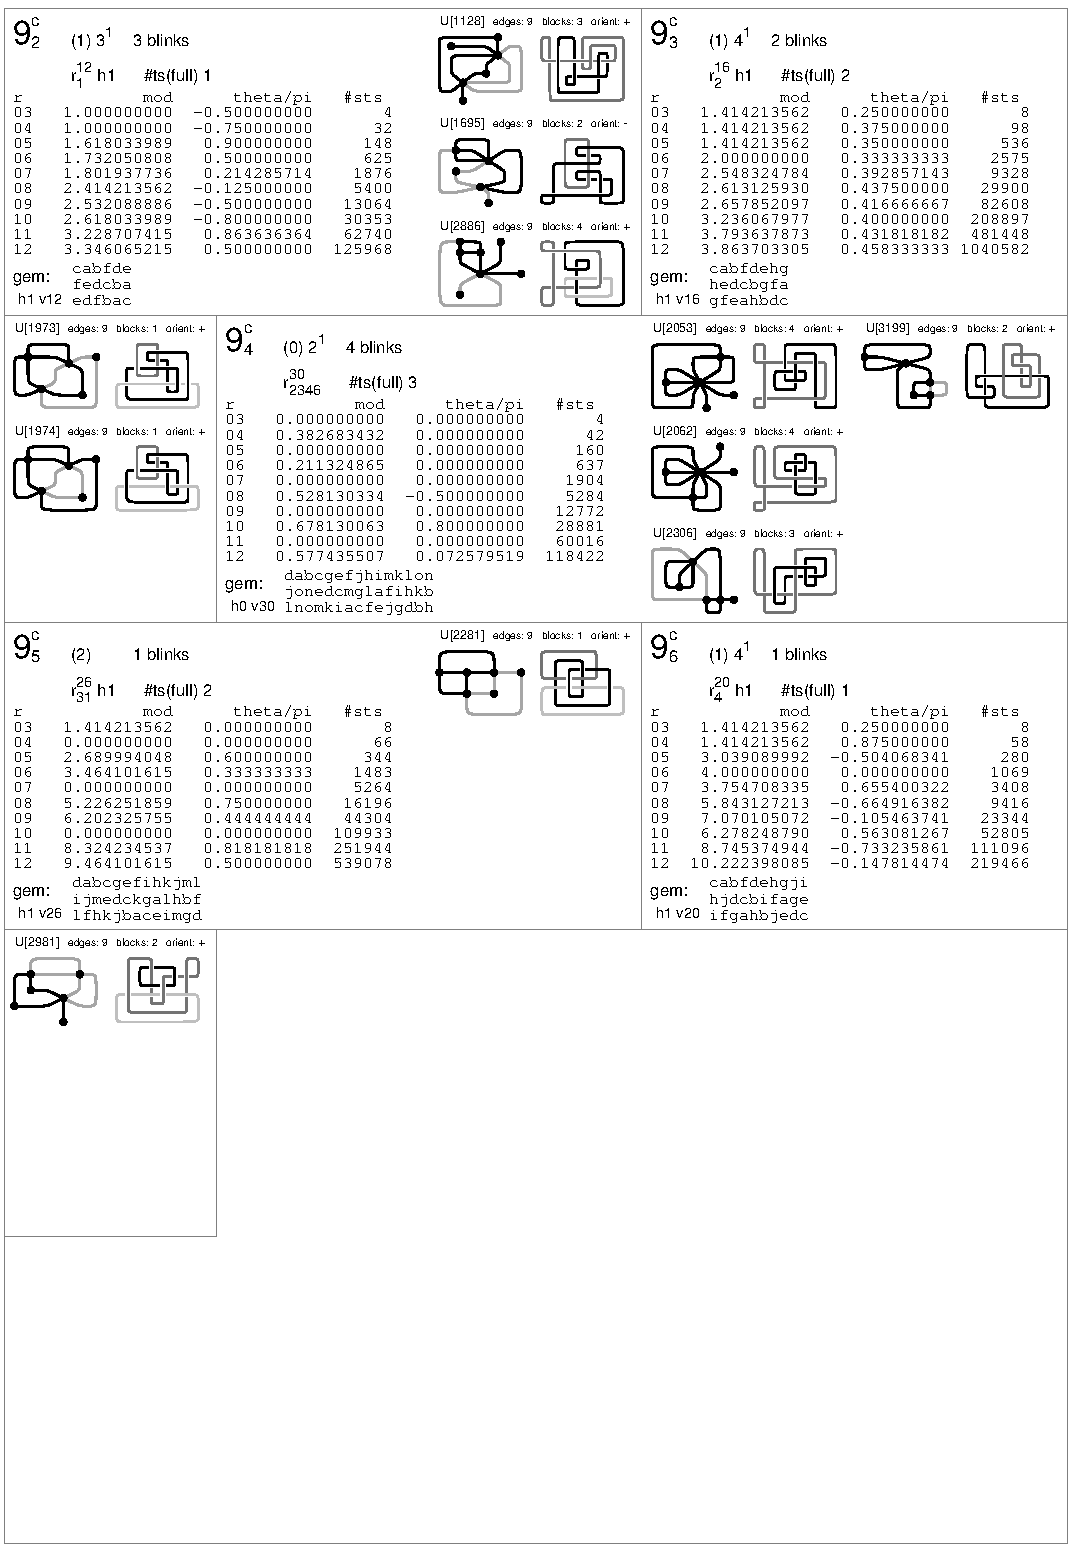
\includegraphics[height=23.5cm]{E.figsbw2/compcatalog003_bw.pdf} \eject
\end{center}